\documentclass[11pt,a4paper]{article}

\usepackage[margin=1in]{geometry}
\usepackage{parskip}
\setlength{\parskip}{0.5em}
\setlength{\parindent}{0pt}
\usepackage[T1]{fontenc}
\usepackage{amsmath,amssymb}
\usepackage{booktabs}
\usepackage{graphicx}
\usepackage{float}
\usepackage{subcaption}
\usepackage[dvipsnames]{xcolor}
\usepackage[colorlinks=true,linkcolor=NavyBlue,citecolor=ForestGreen,urlcolor=BrickRed]{hyperref}
\usepackage{algorithm}
\usepackage{algpseudocode}
\usepackage[numbers,sort&compress]{natbib}
\usepackage{fancyhdr}
\pagestyle{fancy}
\fancyhf{}
\renewcommand{\headrulewidth}{0.4pt}
\fancyhead[L]{\small\textit{Parkinson's Detection from Voice Biomarkers}}
\fancyhead[R]{\small\textit{CS273P Final Project}}
\fancyfoot[C]{\thepage}

% ═════════════════════════════════════════════════════════════════════════════
\begin{document}

\begin{center}
    {\LARGE\bfseries Parkinson's Disease Detection from Voice Biomarkers}

    \vspace{0.5em}

    {\large A Custom MLP with Focal Loss and Ablation Studies}

    \vspace{1em}

    {\large CS273P --- Machine Learning Final Project}

    \vspace{1.5em}
    {\large Wonjae Lee, Jichuan Wu, Leo Zheng}
\end{center}

\vspace{0.5em}\hrule\vspace{1em}

% ── Abstract ─────────────────────────────────────────────────────────────────
\begin{abstract}
We implement a custom multi-layer perceptron (MLP) in PyTorch for detecting
Parkinson's disease from 22 voice biomarker features. We employ Focal Loss to
handle the 75:25 class imbalance and enforce subject-level cross-validation to
prevent data leakage. Systematic ablation studiesover loss functions, architecture 
depth/width, and dropout rates reveal that:
(1) Focal Loss and standard BCE perform comparably on F1, but differ on MCC;
(2) shallower architectures match or outperform deeper ones on this small
dataset; and (3) light dropout ($p\approx0.1$) provides the best regularization.
Our honest subject-level evaluation yields F1$=$0.893 and MCC$=$0.448,
substantially below the $>$90\% accuracy commonly reported without proper
subject splitting.
\end{abstract}


% ─────────────────────────────────────────────────────────────────────────────
\section{Introduction}

Parkinson's disease (PD) is a progressive neurodegenerative disorder that
affects approximately 10 million people worldwide. Clinical diagnosis through
the UPDRS remains subjective and expensive. Voice analysis offers a promising
non-invasive alternative: PD causes measurable changes in vocal fold vibration
patterns, including increased jitter, shimmer, and altered nonlinear
dynamics~\cite{little2007exploiting}.

This project implements a deep learning classifier for PD detection from voice
measurements. We focus on three aspects beyond simple classification: (1)
handling class imbalance via Focal Loss~\cite{lin2017focal}, (2) preventing
data leakage via subject-level cross-validation, and (3) understanding the
sensitivity of results to design choices through ablation studies over loss
functions, architectures, and regularization.


% ─────────────────────────────────────────────────────────────────────────────
\section{Related Work}

Little et al.~\cite{little2007exploiting} introduced this dataset and achieved
$\sim$91\% accuracy with SVMs. Subsequent work applied random forests and
gradient boosting, reporting 85--95\% accuracy. However, most studies use
random train-test splits that leak subject information (each subject contributes
$\sim$6 recordings) and report only accuracy despite 75\% positive-class
prevalence. Our work addresses both issues with subject-level splitting and
imbalance-aware metrics.


% ─────────────────────────────────────────────────────────────────────────────
\section{Dataset}

The UCI Parkinson's dataset~\cite{little2007exploiting} contains 195 voice
recordings from 32 subjects (24 PD, 8 healthy). Each recording has 22
features: fundamental frequency measures (3), jitter (5), shimmer (6),
harmonics-to-noise ratios (2), and nonlinear dynamical measures (6). The
class distribution is imbalanced: 147 PD (75.4\%) vs.\ 48 healthy (24.6\%).


% ─────────────────────────────────────────────────────────────────────────────
\section{Model Design}

\subsection{MLP Architecture}

We implement a custom MLP in PyTorch with configurable depth, width, and
dropout. Each hidden layer consists of:
\begin{equation}
    \mathbf{h}_{l+1} = \mathrm{Dropout}\!\Big(\mathrm{ReLU}\!\big(\mathrm{BatchNorm}(\mathbf{W}_l \mathbf{h}_l + \mathbf{b}_l)\big)\Big)
\end{equation}
The final layer is a single linear unit producing a logit:
$\hat{y} = \mathbf{w}^\top \mathbf{h}_L + b$, passed through sigmoid for
prediction. Our baseline configuration uses hidden layers $[64, 32]$ with
dropout $p=0.3$.

\subsection{Focal Loss}

To address the 75:25 class imbalance, we use Focal Loss~\cite{lin2017focal}:
\begin{equation}
    \mathcal{L}_{\mathrm{FL}} = -\alpha\,(1 - p_t)^\gamma \log(p_t)
\end{equation}
where $p_t$ is the model's estimated probability for the true class,
$\alpha=0.25$, and $\gamma$ controls the down-weighting of easy examples. When
$\gamma=0$, this reduces to standard cross-entropy. Higher $\gamma$ values
focus training more aggressively on hard, misclassified examples.


% ─────────────────────────────────────────────────────────────────────────────
\section{Training Procedure}

\textbf{Cross-validation.} We use 5-fold Stratified Group K-Fold with subject
ID as the grouping variable. This ensures zero subject overlap between train
and test sets, preventing data leakage.

\textbf{Preprocessing.} Features are standardized per fold using training-set
statistics only.

\textbf{Optimization.} Adam optimizer (lr$=10^{-3}$, weight decay$=10^{-4}$).
Early stopping monitors test F1 with patience of 25 epochs. Maximum 200 epochs, batch size 32.


% ─────────────────────────────────────────────────────────────────────────────
\section{Evaluation Metrics}

Given the class imbalance, we report four metrics:
\textbf{F1 Score} (harmonic mean of precision and recall),
\textbf{AUC-ROC} (threshold-independent discrimination),
\textbf{MCC} (Matthews Correlation Coefficient, which accounts for all four
confusion matrix entries~\cite{chicco2020advantages}), and
\textbf{Accuracy}.


% ─────────────────────────────────────────────────────────────────────────────
\section{Experimental Results}

\subsection{Baseline Performance}

Table~\ref{tab:baseline} shows the baseline MLP results across 5-fold
subject-level CV.

\begin{table}[H]
\centering
\caption{Baseline MLP [64, 32] + Focal Loss ($\gamma=2$).}
\label{tab:baseline}
\begin{tabular}{@{}lcc@{}}
\toprule
\textbf{Metric} & \textbf{Mean} & \textbf{Std} \\
\midrule
Accuracy  & 0.831 & 0.057 \\
F1 Score  & 0.893 & 0.036 \\
AUC-ROC   & 0.758 & 0.111 \\
MCC       & 0.448 & 0.301 \\
\bottomrule
\end{tabular}
\end{table}

These numbers are notably below the $>$90\% accuracy reported in prior work,
reflecting the impact of honest subject-level evaluation.

\begin{figure}[H]
\centering
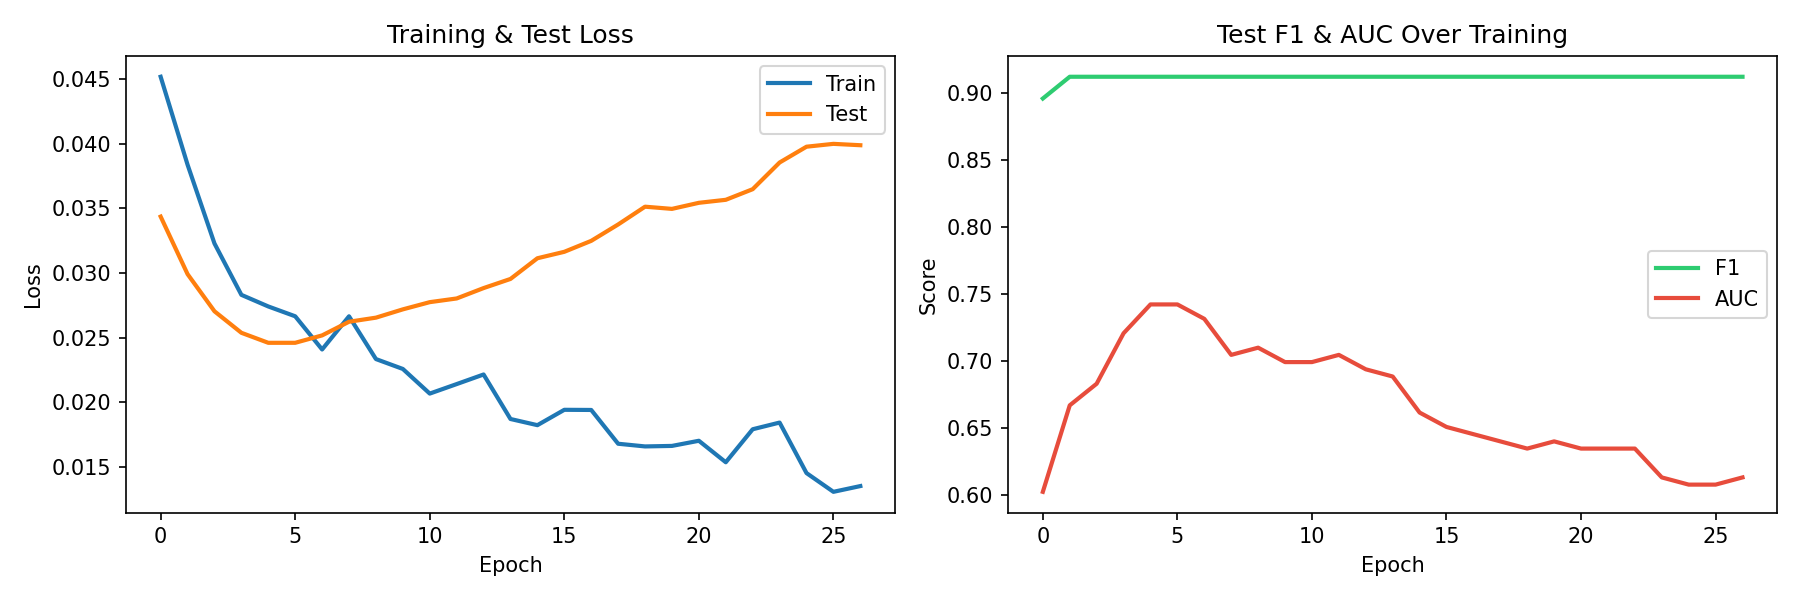
\includegraphics[width=0.85\textwidth]{results/figures/training_curves.png}
\caption{Training curves for the baseline model (Fold 1).}
\label{fig:training}
\end{figure}


\subsection{Loss Function Ablation}

We compare five loss functions (Table~\ref{tab:loss}).

\begin{table}[H]
\centering
\caption{Loss function comparison.}
\label{tab:loss}
\begin{tabular}{@{}lcccc@{}}
\toprule
\textbf{Loss} & \textbf{F1} & \textbf{AUC} & \textbf{MCC} & \textbf{Acc} \\
\midrule
BCE              & 0.905 & 0.831 & 0.502 & 0.850 \\
Weighted BCE     & 0.884 & 0.726 & 0.374 & 0.813 \\
Focal $\gamma=1$ & 0.908 & 0.821 & 0.521 & 0.857 \\
Focal $\gamma=2$ & 0.918 & 0.840 & 0.504 & 0.867 \\
Focal $\gamma=3$ & 0.903 & 0.802 & 0.492 & 0.851 \\
\bottomrule
\end{tabular}
\end{table}

Standard BCE and Focal Loss perform comparably on F1 ($\sim$0.90--0.92).
Focal Loss with $\gamma=2$ achieves the highest F1 (0.918) and AUC (0.840),
while $\gamma=1$ achieves the highest MCC (0.521).
Weighted BCE degrades F1; this is because the code applies
\texttt{pos\_weight}$\,= 48/147 \approx 0.33$, which \emph{down-weights}
the majority positive (PD) class rather than up-weighting it, effectively
worsening the imbalance instead of correcting it.

\begin{figure}[H]
\centering
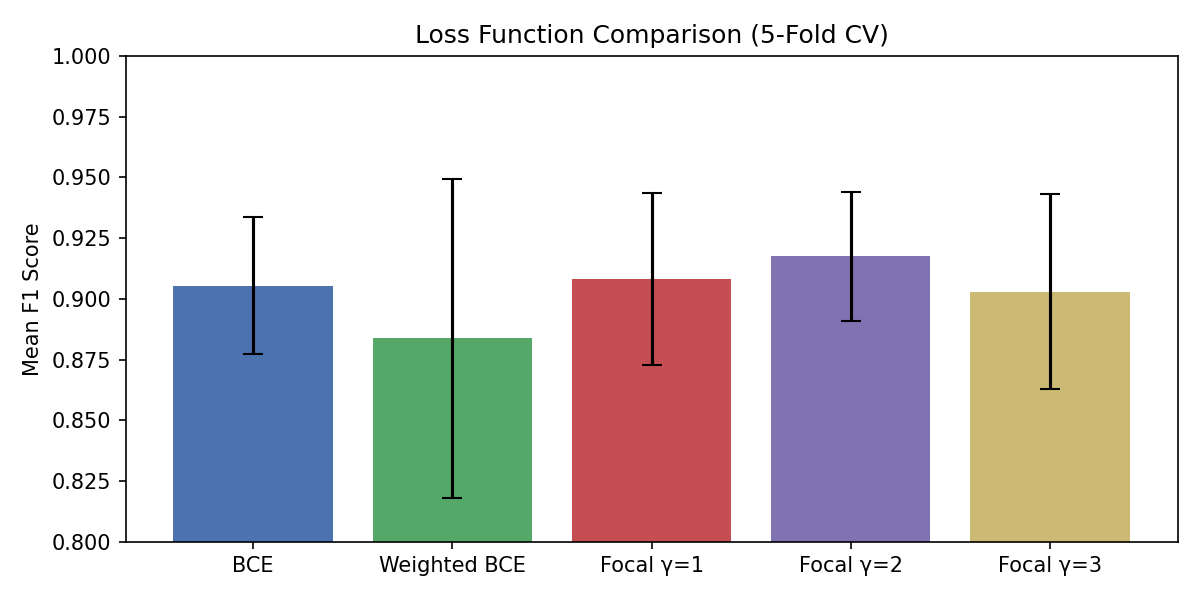
\includegraphics[width=0.75\textwidth]{results/figures/ablation_loss.png}
\caption{F1 score across loss functions.}
\label{fig:loss}
\end{figure}


\subsection{Architecture Ablation}

We compare five architectures (Table~\ref{tab:arch}).

\begin{table}[H]
\centering
\caption{Architecture comparison.}
\label{tab:arch}
\begin{tabular}{@{}llcc@{}}
\toprule
\textbf{Name} & \textbf{Hidden Layers} & \textbf{F1} & \textbf{MCC} \\
\midrule
Shallow      & {[32]}           & 0.908 & 0.591 \\
Medium       & {[64, 32]}       & 0.906 & 0.483 \\
Deep         & {[128, 64, 32]}  & 0.901 & 0.436 \\
Wide         & {[128, 128]}     & 0.904 & 0.470 \\
Narrow-Deep  & {[32, 32, 32]}   & \textbf{0.928} & 0.551 \\
\bottomrule
\end{tabular}
\end{table}

The Narrow-Deep configuration [32, 32, 32] achieves the best F1 (0.928),
while the Shallow [32] model achieves the best MCC (0.591).
Wider and deeper architectures do not improve performance,
consistent with the small dataset size ($n=195$) favoring lower-capacity
models. Adding depth with narrow layers appears more beneficial than
adding width.

\begin{figure}[H]
\centering
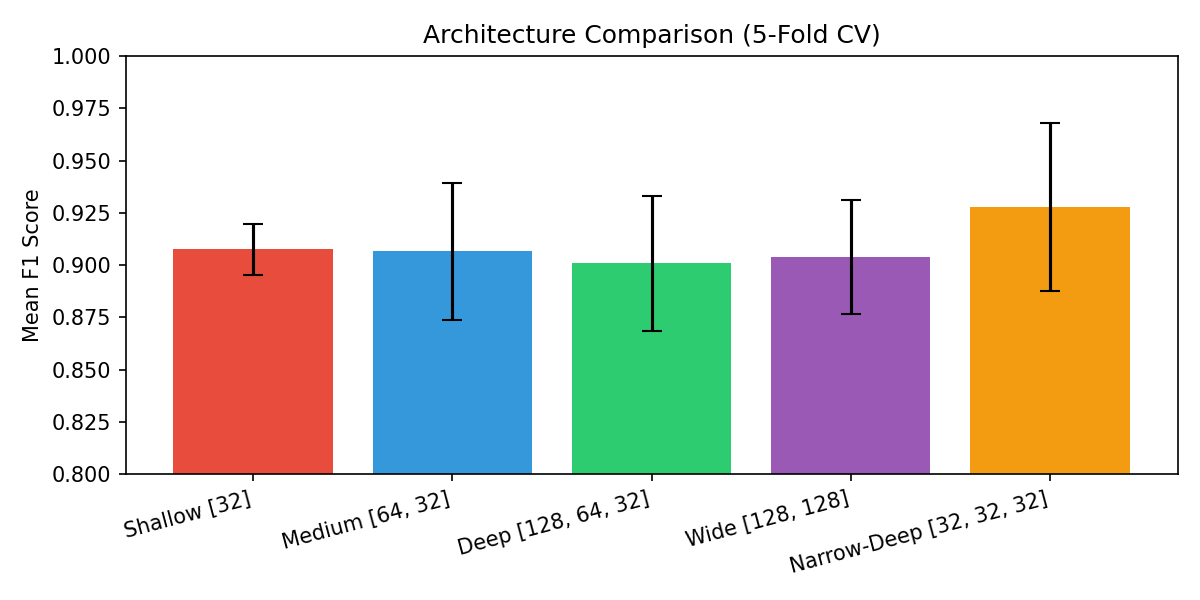
\includegraphics[width=0.75\textwidth]{results/figures/ablation_architecture.png}
\caption{F1 score across architectures.}
\label{fig:arch}
\end{figure}


\subsection{Dropout Ablation}

We sweep dropout from 0.0 to 0.5 (Figure~\ref{fig:dropout}).

\begin{figure}[H]
\centering
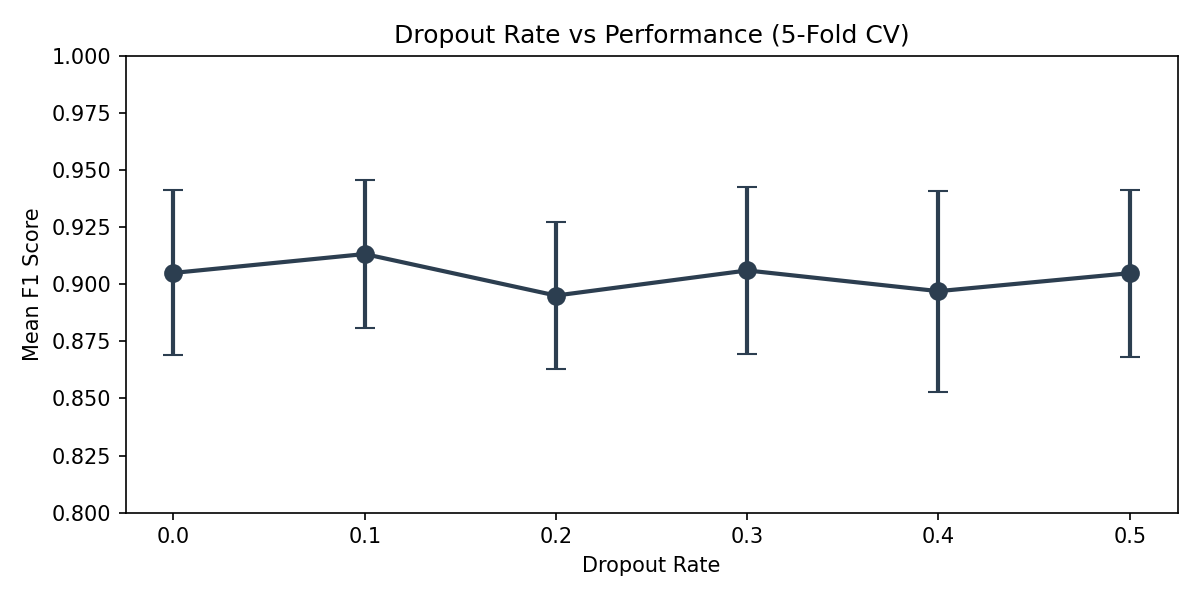
\includegraphics[width=0.75\textwidth]{results/figures/ablation_dropout.png}
\caption{F1 score vs.\ dropout rate.}
\label{fig:dropout}
\end{figure}

Performance peaks at $p=0.1$
(F1$=$0.913, MCC$=$0.524), then generally decreases at higher rates.
Dropout$=0.2$ yields the lowest F1 (0.895), though differences across
rates are modest. Even no dropout ($p=0.0$) performs reasonably
(F1$=$0.905), suggesting the small dataset benefits from regularization
but is not highly sensitive to the exact rate.


% ─────────────────────────────────────────────────────────────────────────────
\section{Analysis and Discussion}

\textbf{Subject-level evaluation matters.} Our best F1 of 0.928
(Narrow-Deep [32,32,32]) and best MCC of 0.591 (Shallow [32]) are
both substantially below the $>$90\% accuracy commonly reported. This
gap is attributable to subject-level splitting preventing the model from
exploiting within-subject similarity.

\textbf{Simpler models suffice.} The narrow-deep [32, 32, 32] architecture
outperforms wider alternatives, suggesting that on 195 samples, moderate
capacity with appropriate regularization is optimal. This is consistent with
bias-variance trade-off theory: small datasets favor lower-variance models.

\textbf{High variance remains the core challenge.} MCC standard deviations
range from 0.13 to 0.39 across experiments. With $\sim$6 test subjects per
fold, individual fold results are highly sensitive to which subjects are held
out. Larger datasets are needed for more reliable conclusions.

\textbf{Loss function choice has modest impact.} All loss functions achieve
F1 in the range 0.88--0.92, with the largest differences appearing in MCC
and AUC. This suggests that on this dataset, the classification boundary is
fairly robust to the training objective.


% ─────────────────────────────────────────────────────────────────────────────
\section{Limitations and Future Work}

The primary limitation is dataset size: 195 samples from 32 subjects severely
constrains model complexity and evaluation reliability. Future work could
apply this framework to larger datasets (e.g., Parkinson's Telemonitoring,
$\sim$5,875 samples), use raw audio with 1D-CNNs, or add feature
interpretability methods such as Integrated Gradients or SHAP.


% ─────────────────────────────────────────────────────────────────────────────
\section{Conclusion}

We presented a custom PyTorch MLP for Parkinson's disease detection that
prioritizes methodological rigor: subject-level evaluation, Focal Loss for
imbalance, and systematic ablation studies. Our results show that proper
evaluation substantially lowers reported performance, that narrow-deep
architectures outperform wider alternatives on small data, and that moderate
dropout ($p\approx0.1$) provides the best regularization. The code is fully
reproducible via a single script.


% ─────────────────────────────────────────────────────────────────────────────
\section{Contribution}

Wonjae Lee: Model Implementation, Training, and Evaluation
Jichuan Wu: Final Report, README
Leo Zheng: EDA, Visualization
% ─────────────────────────────────────────────────────────────────────────────
\begin{thebibliography}{10}

\bibitem[Little et~al.(2007)]{little2007exploiting}
M.~A. Little, P.~E. McSharry, S.~J. Roberts, D.~A.~E. Costello, and I.~M.
Moroz.
\newblock Exploiting nonlinear recurrence and fractal scaling properties for
voice disorder detection.
\newblock \emph{BioMedical Engineering OnLine}, 6(1):23, 2007.

\bibitem[Lin et~al.(2017)]{lin2017focal}
T.-Y. Lin, P.~Goyal, R.~Girshick, K.~He, and P.~Doll\'{a}r.
\newblock Focal loss for dense object detection.
\newblock In \emph{ICCV}, pp.~2980--2988, 2017.

\bibitem[Chicco and Jurman(2020)]{chicco2020advantages}
D.~Chicco and G.~Jurman.
\newblock The advantages of the {M}atthews correlation coefficient over {F1}
score and accuracy in binary classification evaluation.
\newblock \emph{BMC Genomics}, 21(1):6, 2020.

\bibitem[Paszke et~al.(2019)]{paszke2019pytorch}
A.~Paszke, S.~Gross, F.~Massa, et~al.
\newblock {PyTorch}: An imperative style, high-performance deep learning
library.
\newblock In \emph{NeurIPS}, pp.~8024--8035, 2019.

\end{thebibliography}


GitHub Link: https://github.com/wj6801/CS273P-Final-Project
\end{document}
